% Fix: From https://tex.stackexchange.com/a/508995/108670
\RequirePackage{snapshot}
\makeatletter
\def\snap@providesfile#1[#2]{%
    \wlog{File: #1 #2}%
    \if\expandafter\snap@graphic@test\expanded{#2}@@\@nil
    \snap@record@graphic#1\relax #2 (type ??)\@nil
    \else
    \expandafter\xdef\csname ver@#1\endcsname{#2}%
    \fi
    \endgroup
}
\makeatother

%\pgfplotsset{compat=1.18}
\documentclass[twoside,a4paper,11pt]{memoir}
\usepackage{document}
\usepackage[hidelinks]{hyperref}
\usepackage[noabbrev, nameinlink]{cleveref}
\usepackage{tikz}
\usepackage{pgfplots}
\usepackage[outputdir=../out]{minted}
\usepackage{listings-rust}
\usepackage{codex}
\usepackage{subcaption}
\usepackage{float}
\usepackage{fontawesome5}

\usetikzlibrary{%
    arrows,%
    calc,%
    fit,%
    patterns,%
    plotmarks,%
    shapes.geometric,%
    shapes.misc,%
    shapes.symbols,%
    shapes.arrows,%
    shapes.callouts,%
% shapes.multipart,%
% shapes.gates.logic.US,%
% shapes.gates.logic.IEC,%
% er,%
% automata,%
    backgrounds,%
    chains,%
    topaths,%
    trees,%
    petri,%
    mindmap,%
    matrix,%
% calendar,%
    folding,%
    fadings,%
    through,%
    positioning,%
    scopes,%
    decorations.fractals,%
    decorations.shapes,%
    decorations.text,%
    decorations.pathmorphing,%
    decorations.pathreplacing,%
    decorations.footprints,%
    decorations.markings,%
    shadows}
\newfontfamily\xkcd{xkcd}

\newfloat{lstfloat}{htbp}{lop}
\floatname{lstfloat}{Listing}
\def\lstfloatautorefname{Listing}

\newcommand{\problem}[1]{$m #1 n$}

% Add \@ _before_ the terminating period of the sentence (`UI\@. Test`)
% to allow inter-sentence spacing when the sentence ends with a capital letter.

\addbibresource{document.bib}
\addbibresource{researchr.bib}

% !TEX root = document.tex

\title{A generic format for code viewer services}
\subtitle{Version of \today}
%\subtitle{Master's Thesis}
\author{Jonathan Dönszelmann}
\authoremail{\url{j.b.donszelmann@student.tudelft.nl}}
\birthplace{Amsterdam, the Netherlands}
\studentid{4888766}
\coverpicture{
\includegraphics[width=13cm]{./img/maze.ps}}
\colophon{\noindent
  \copyright{} \the\year{} \: \theauthor. \\[1em]
  Cover picture: Random maze.
}



\begin{document}

    
\definecolor{color60}{RGB}{227,98,9}
\definecolor{color59}{RGB}{215,58,73}
\definecolor{color61}{RGB}{0,92,197}
\definecolor{color58}{RGB}{36,41,46}
\definecolor{vbackground}{RGB}{255,255,255}
\definecolor{vforeground}{RGB}{36,41,46}

\newcommand\codePaperExampleElaine{

    \begin{codexcode}
        {\color{color59}use}{\color{color58}\enspace }{\color{color60}std}{\color{color58};}\leavevmode \\
\leavevmode \\
{\color{color59}effect}{\color{color58}\enspace }\hyperlink{goto1565}{\color{vforeground}\underline{\linkdest{goto175}{}{\color{color60}Abort}}}{\color{color58}\enspace \{}\leavevmode \\
{\color{color58}\enspace \enspace }\hyperlink{goto1895}{\color{vforeground}\underline{\linkdest{goto275}{}{\color{color60}abort}}}{\color{color58}()\enspace }{\color{color59}a}\leavevmode \\
{\color{color58}\}}\leavevmode \\
\leavevmode \\
{\color{color59}let}{\color{color58}\enspace }\linkdest{goto446}{}{\color{color60}hAbort}\textsuperscript{\hyperlink{goto2556}{\color{vforeground}usag,}}\textsuperscript{\hyperlink{goto2916}{\color{vforeground}usag}}{\color{color58}\enspace =\enspace }{\color{color59}fn}{\color{color58}(}\hyperlink{goto1137}{\color{vforeground}\underline{\linkdest{goto567}{}{\color{color60}default}}}{\color{color58})\enspace \{}\leavevmode \\
{\color{color58}\enspace \enspace }{\color{color59}handler}{\color{color58}\enspace \{}\leavevmode \\
{\color{color58}\enspace \enspace \enspace \enspace }{\color{color59}return}{\color{color58}(}\hyperlink{goto951}{\color{vforeground}\underline{\linkdest{goto901}{}{\color{color60}x}}}{\color{color58})\enspace \{\enspace }\hyperlink{goto901}{\color{vforeground}\underline{\linkdest{goto951}{}{\color{color60}x}}}{\color{color58}\enspace \}}\leavevmode \\
{\color{color58}\enspace \enspace \enspace \enspace }{\color{color60}abort}{\color{color58}()\enspace \{\enspace }\hyperlink{goto567}{\color{vforeground}\underline{\linkdest{goto1137}{}{\color{color60}default}}}{\color{color58}\enspace \}}\leavevmode \\
{\color{color58}\enspace \enspace \}}\leavevmode \\
{\color{color58}\};}\leavevmode \\
\leavevmode \\
{\color{color59}let}{\color{color58}\enspace }\linkdest{goto1358}{}{\color{color60}safe\_div}\textsuperscript{\hyperlink{goto2668}{\color{vforeground}usag,}}\textsuperscript{\hyperlink{goto3028}{\color{vforeground}usag}}{\color{color58}\enspace =\enspace }{\color{color59}fn}{\color{color58}(}\hyperlink{goto2161}{\color{vforeground}\underline{\linkdest{goto1491}{}{\color{color60}x}}}{\color{color58},\enspace }\linkdest{goto1521}{}{\color{color60}y}\textsuperscript{\hyperlink{goto1771}{\color{vforeground}usag,}}\textsuperscript{\hyperlink{goto2191}{\color{vforeground}usag}}{\color{color58})\enspace <}\hyperlink{goto175}{\color{vforeground}\underline{\linkdest{goto1565}{}{\color{color60}Abort}}}{\color{color58}>\enspace }{\color{color59}Int}{\color{color58}\enspace \{}\leavevmode \\
{\color{color58}\enspace \enspace }{\color{color59}if}{\color{color58}\enspace }{\color{color60}eq}{\color{color58}(}\hyperlink{goto1521}{\color{vforeground}\underline{\linkdest{goto1771}{}{\color{color60}y}}}{\color{color58},\enspace }{\color{color61}0}{\color{color58})\enspace \{}\leavevmode \\
{\color{color58}\enspace \enspace \enspace \enspace }\hyperlink{goto275}{\color{vforeground}\underline{\linkdest{goto1895}{}{\color{color60}abort}}}{\color{color58}()}\leavevmode \\
{\color{color58}\enspace \enspace \}\enspace }{\color{color59}else}{\color{color58}\enspace \{}\leavevmode \\
{\color{color58}\enspace \enspace \enspace \enspace }{\color{color60}div}{\color{color58}(}\hyperlink{goto1491}{\color{vforeground}\underline{\linkdest{goto2161}{}{\color{color60}x}}}{\color{color58},\enspace }\hyperlink{goto1521}{\color{vforeground}\underline{\linkdest{goto2191}{}{\color{color60}y}}}{\color{color58})}\leavevmode \\
{\color{color58}\enspace \enspace \}}\leavevmode \\
{\color{color58}\};}\leavevmode \\
\leavevmode \\
{\color{color59}let}{\color{color58}\enspace }{\color{color60}main}{\color{color58}\enspace =\enspace }{\color{color60}add}{\color{color58}(}\leavevmode \\
{\color{color58}\enspace \enspace }{\color{color59}handle}{\color{color58}[}\hyperlink{goto446}{\color{vforeground}\underline{\linkdest{goto2556}{}{\color{color60}hAbort}}}{\color{color58}(}{\color{color61}0}{\color{color58})]\enspace }\hyperlink{goto1358}{\color{vforeground}\underline{\linkdest{goto2668}{}{\color{color60}safe\_div}}}{\color{color58}(}{\color{color61}3}{\color{color58},\enspace }{\color{color61}0}{\color{color58}),}\leavevmode \\
{\color{color58}\enspace \enspace }{\color{color59}handle}{\color{color58}[}\hyperlink{goto446}{\color{vforeground}\underline{\linkdest{goto2916}{}{\color{color60}hAbort}}}{\color{color58}(}{\color{color61}0}{\color{color58})]\enspace }\hyperlink{goto1358}{\color{vforeground}\underline{\linkdest{goto3028}{}{\color{color60}safe\_div}}}{\color{color58}(}{\color{color61}10}{\color{color58},\enspace }{\color{color61}2}{\color{color58}),}\leavevmode \\
{\color{color58});}
    \end{codexcode}
}


    
\definecolor{colorfield3}{RGB}{111,66,193}
\definecolor{colorfield0}{RGB}{36,41,46}
\definecolor{colorfield1}{RGB}{106,115,125}
\definecolor{colorfield2}{RGB}{215,58,73}
\definecolor{colorfield4}{RGB}{227,98,9}
\definecolor{vbackground}{RGB}{255,255,255}
\definecolor{vforeground}{RGB}{36,41,46}

\newcommand\codeDataStructuresRs{

    \begin{codexcode}
        {\color{colorfield1}//\enspace \allowbreak Types}\leavevmode \\
\linkdest{goto4668}{}{\color{colorfield2}struct}{\color{colorfield0}\enspace \allowbreak }{\color{colorfield3}Span}{\color{colorfield0}\enspace \allowbreak }{\color{colorfield0}\{}\leavevmode \\
{\color{colorfield0}\enspace \allowbreak \enspace \allowbreak \enspace \allowbreak \enspace \allowbreak }\linkdest{goto6412}{}{\color{colorfield4}start}{\color{colorfield2}:}{\color{colorfield0}\enspace \allowbreak }{\color{colorfield3}usize}{\color{colorfield0},}\leavevmode \\
{\color{colorfield0}\enspace \allowbreak \enspace \allowbreak \enspace \allowbreak \enspace \allowbreak }\linkdest{goto8213}{}{\color{colorfield4}length}{\color{colorfield2}:}{\color{colorfield0}\enspace \allowbreak }{\color{colorfield3}usize}{\color{colorfield0},}\leavevmode \\
{\color{colorfield0}\enspace \allowbreak \enspace \allowbreak \enspace \allowbreak \enspace \allowbreak }\linkdest{goto10110}{}{\color{colorfield4}file}{\color{colorfield2}:}{\color{colorfield0}\enspace \allowbreak }{\color{colorfield3}Path}{\color{colorfield0},}\leavevmode \\
{\color{colorfield0}\}}\leavevmode \\
\linkdest{goto144}{}{\color{colorfield2}s}{\color{colorfield2}truct}{\color{colorfield0}\enspace \allowbreak }{\color{colorfield3}Classification}{\color{colorfield0}(}{\color{colorfield3}Vec}{\color{colorfield0}<}{\color{colorfield3}String}{\color{colorfield0}>}{\color{colorfield0})}{\color{colorfield0};}\leavevmode \\
\linkdest{goto11520}{}{\color{colorfield2}struct}{\color{colorfield0}\enspace \allowbreak }{\color{colorfield3}Text}{\color{colorfield0}(}{\color{colorfield3}String}{\color{colorfield0})}{\color{colorfield0};}\leavevmode \\
\leavevmode \\
\linkdest{goto137305}{}{\color{colorfield1}//\enspace \allowbreak Relations}\leavevmode \\
{\color{colorfield2}enum}{\color{colorfield0}\enspace \allowbreak }{\color{colorfield3}Relation}{\color{colorfield0}\enspace \allowbreak }{\color{colorfield0}\{}\leavevmode \\
{\color{colorfield0}\enspace \allowbreak \enspace \allowbreak \enspace \allowbreak \enspace \allowbreak }\linkdest{goto17067}{}{\color{colorfield3}Outline}{\color{colorfield0}\enspace \allowbreak }{\color{colorfield0}\{}\leavevmode \\
{\color{colorfield0}\enspace \allowbreak \enspace \allowbreak \enspace \allowbreak \enspace \allowbreak \enspace \allowbreak \enspace \allowbreak \enspace \allowbreak \enspace \allowbreak }\linkdest{goto18820}{}{\color{colorfield4}kind}{\color{colorfield2}:}{\color{colorfield0}\enspace \allowbreak }\hyperlink{goto144}{\color{vforeground}\underline{{\color{colorfield3}Classification}}}{\color{colorfield0},}\leavevmode \\
{\color{colorfield0}\enspace \allowbreak \enspace \allowbreak \enspace \allowbreak \enspace \allowbreak \enspace \allowbreak \enspace \allowbreak \enspace \allowbreak \enspace \allowbreak }\linkdest{goto21812}{}{\color{colorfield4}parent}{\color{colorfield2}:}{\color{colorfield0}\enspace \allowbreak }\hyperlink{goto4668}{\color{vforeground}\underline{{\color{colorfield3}Span}}}{\color{colorfield0},}\leavevmode \\
{\color{colorfield0}\enspace \allowbreak \enspace \allowbreak \enspace \allowbreak \enspace \allowbreak }{\color{colorfield0}\}}{\color{colorfield0},}\leavevmode \\
{\color{colorfield0}\enspace \allowbreak \enspace \allowbreak \enspace \allowbreak \enspace \allowbreak }\linkdest{goto24344}{}{\color{colorfield3}Syntax}{\color{colorfield0}\enspace \allowbreak }{\color{colorfield0}\{}\leavevmode \\
{\color{colorfield0}\enspace \allowbreak \enspace \allowbreak \enspace \allowbreak \enspace \allowbreak \enspace \allowbreak \enspace \allowbreak \enspace \allowbreak \enspace \allowbreak }\linkdest{goto26020}{}{\color{colorfield4}kind}{\color{colorfield2}:}{\color{colorfield0}\enspace \allowbreak }\hyperlink{goto144}{\color{vforeground}\underline{{\color{colorfield3}Classification}}}{\color{colorfield0},}\leavevmode \\
{\color{colorfield0}\enspace \allowbreak \enspace \allowbreak \enspace \allowbreak \enspace \allowbreak }{\color{colorfield0}\}}{\color{colorfield0},}\leavevmode \\
{\color{colorfield0}\enspace \allowbreak \enspace \allowbreak \enspace \allowbreak \enspace \allowbreak }\linkdest{goto29369}{}{\color{colorfield3}Reference}{\color{colorfield0}\enspace \allowbreak }{\color{colorfield0}\{}\leavevmode \\
{\color{colorfield0}\enspace \allowbreak \enspace \allowbreak \enspace \allowbreak \enspace \allowbreak \enspace \allowbreak \enspace \allowbreak \enspace \allowbreak \enspace \allowbreak }\linkdest{goto31312}{}{\color{colorfield4}target}{\color{colorfield2}:}{\color{colorfield0}\enspace \allowbreak }\hyperlink{goto4668}{\color{vforeground}\underline{{\color{colorfield3}Span}}}{\color{colorfield0},}\leavevmode \\
{\color{colorfield0}\enspace \allowbreak \enspace \allowbreak \enspace \allowbreak \enspace \allowbreak \enspace \allowbreak \enspace \allowbreak \enspace \allowbreak \enspace \allowbreak }\linkdest{goto33520}{}{\color{colorfield4}kind}{\color{colorfield2}:}{\color{colorfield0}\enspace \allowbreak }\hyperlink{goto144}{\color{vforeground}\underline{{\color{colorfield3}Classification}}}{\color{colorfield0},}\leavevmode \\
{\color{colorfield0}\enspace \allowbreak \enspace \allowbreak \enspace \allowbreak \enspace \allowbreak }{\color{colorfield0}\}}{\color{colorfield0},}\leavevmode \\
{\color{colorfield0}\enspace \allowbreak \enspace \allowbreak \enspace \allowbreak \enspace \allowbreak }\linkdest{goto36872}{}{\color{colorfield3}Diagnostics}{\color{colorfield0}\enspace \allowbreak }{\color{colorfield0}\{}\leavevmode \\
{\color{colorfield0}\enspace \allowbreak \enspace \allowbreak \enspace \allowbreak \enspace \allowbreak \enspace \allowbreak \enspace \allowbreak \enspace \allowbreak \enspace \allowbreak }\linkdest{goto39020}{}{\color{colorfield4}kind}{\color{colorfield2}:}{\color{colorfield0}\enspace \allowbreak }\hyperlink{goto144}{\color{vforeground}\underline{{\color{colorfield3}Classification}}}{\color{colorfield0},}\leavevmode \\
{\color{colorfield0}\enspace \allowbreak \enspace \allowbreak \enspace \allowbreak \enspace \allowbreak \enspace \allowbreak \enspace \allowbreak \enspace \allowbreak \enspace \allowbreak }\linkdest{goto42013}{}{\color{colorfield4}message}{\color{colorfield2}:}{\color{colorfield0}\enspace \allowbreak }\hyperlink{goto11520}{\color{vforeground}\underline{{\color{colorfield3}Text}}}{\color{colorfield0},}\leavevmode \\
{\color{colorfield0}\enspace \allowbreak \enspace \allowbreak \enspace \allowbreak \enspace \allowbreak }{\color{colorfield0}\}}\leavevmode \\
{\color{colorfield0}\}}\leavevmode \\
\leavevmode \\
\linkdest{goto44450}{}{\color{colorfield1}//\enspace \allowbreak Metadata}\leavevmode \\
{\color{colorfield2}type}{\color{colorfield0}\enspace \allowbreak }{\color{colorfield3}Metadata}{\color{colorfield0}\enspace \allowbreak }{\color{colorfield2}=}{\color{colorfield0}\enspace \allowbreak }{\color{colorfield3}Vec}{\color{colorfield0}<}{\color{colorfield0}(}\hyperlink{goto4668}{\color{vforeground}\underline{{\color{colorfield3}Span}}}{\color{colorfield0},}{\color{colorfield0}\enspace \allowbreak }\hyperlink{goto137305}{\color{vforeground}\underline{{\color{colorfield3}Relation}}}{\color{colorfield0})}{\color{colorfield0}>}{\color{colorfield0};}
    \end{codexcode}
}


    \definecolor{color20}{RGB}{36,41,46}
\definecolor{color9}{RGB}{111,66,193}
\definecolor{color12}{RGB}{215,58,73}
\definecolor{color8}{RGB}{3,47,98}
\definecolor{color126}{RGB}{227,98,9}
\definecolor{vbackground}{RGB}{255,255,255}
\definecolor{vforeground}{RGB}{36,41,46}

\newcommand\codeBRs{

    \begin{codexcode}
        \linkdest{goto2864}{}{\color{color12}fn}{\color{color20}\enspace }{\color{color9}print\_square}{\color{color20}(}\linkdest{goto441}{}{\color{color126}n}{\color{color12}:}{\color{color20}\enspace }\linkdest{goto476}{}{\color{color9}Number}\textsuperscript{\hyperlink{goto058}{\color{vforeground}decl,}}\textsuperscript{\hyperlink{goto016}{\color{vforeground}impl,}}\textsuperscript{\hyperlink{goto986}{\color{vforeground}usag,}}\textsuperscript{\hyperlink{goto1364}{\color{vforeground}usag}}{\color{color20})}{\color{color20}\enspace \{}\leavevmode \\
\linkdest{goto566}{}{\color{color20}\enspace \enspace \enspace \enspace }{\color{color9}p}{\color{color9}rin}{\color{color9}tln!}{\color{color20}(}{\color{color8}"}{\color{color8}\{}{\color{color8}:?}{\color{color8}\}}{\color{color8}"}\linkdest{goto766}{}{\color{color20},}{\color{color20}\enspace }\hyperlink{goto441}{\color{vforeground}\underline{\linkdest{goto781}{}{\color{color126}n}}}{\color{color12}.}\hyperlink{goto19370}{\color{vforeground}\underline{{\color{color9}square}}}{\color{color20}(}{\color{color20})}{\color{color20})}{\color{color20};}\leavevmode \\
{\color{color20}\}}\leavevmode \\
\leavevmode \\

    \end{codexcode}
}

\newcommand\codeNumberRs{

    \begin{codexcode}
        \linkdest{goto058}{}\linkdest{goto054}{}\linkdest{goto016}{}{\color{color20}\#}{\color{color20}[}{\color{color20}derive}{\color{color20}(}{\color{color9}Debug}{\color{color20})}{\color{color20}]}\leavevmode \\
{\color{color12}pub}{\color{color20}\enspace }{\color{color12}struct}{\color{color20}\enspace }{\color{color9}Number}\textsuperscript{\hyperlink{goto016}{\color{vforeground}impl,}}\textsuperscript{\hyperlink{goto56209}{\color{vforeground}impl,}}\textsuperscript{\hyperlink{goto566}{\color{vforeground}usag}}{\color{color20}\enspace }{\color{color20}\{}\leavevmode \\
{\color{color20}\enspace \enspace \enspace \enspace }\linkdest{goto4110}{}{\color{color126}inner}{\color{color12}:}{\color{color20}\enspace }{\color{color9}u32}{\color{color20},}\leavevmode \\
{\color{color20}\}}\leavevmode \\
\leavevmode \\
\linkdest{goto56209}{}{\color{color12}im}{\color{color12}pl}{\color{color20}\enspace }\linkdest{goto616}{}{\color{color9}Number}\textsuperscript{\hyperlink{goto054}{\color{vforeground}decl,}}\textsuperscript{\hyperlink{goto016}{\color{vforeground}impl,}}\textsuperscript{\hyperlink{goto566}{\color{vforeground}usag}}{\color{color20}\enspace }{\color{color20}\{}\leavevmode \\
{\color{color20}\enspace \enspace \enspace \enspace }\linkdest{goto74113}{}{\color{color12}pub}{\color{color20}\enspace }{\color{color12}fn}{\color{color20}\enspace }{\color{color9}multiply}{\color{color20}(}\linkdest{goto905}{}{\color{color12}\&}{\color{color126}self}{\color{color20},}{\color{color20}\enspace }\linkdest{goto975}{}{\color{color126}o}\linkdest{goto986}{}{\color{color126}ther}{\color{color12}:}{\color{color20}\enspace }{\color{color9}u32}{\color{color20})}{\color{color20}\enspace }{\color{color12}->}{\color{color20}\enspace }\linkdest{goto1124}{}{\color{color126}Self}{\color{color20}\enspace \{}\leavevmode \\
{\color{color20}\enspace \enspace \enspace \enspace \enspace \enspace \enspace \enspace }\linkdest{goto1274}{}{\color{color126}Self}{\color{color20}\enspace }{\color{color20}\{}\leavevmode \\
{\color{color20}\enspace \enspace }\linkdest{goto1364}{}{\color{color20}\enspace \enspace \enspace \enspace }{\color{color20}\enspace \enspace \enspace \enspace \enspace \enspace }\hyperlink{goto4110}{\color{vforeground}\underline{\linkdest{goto1465}{}{\color{color126}inner}}}{\color{color12}:}{\color{color20}\enspace }\hyperlink{goto905}{\color{vforeground}\underline{\linkdest{goto1534}{}{\color{color126}self}}}{\color{color12}.}\hyperlink{goto4110}{\color{vforeground}\underline{\linkdest{goto1585}{}{\color{color126}inner}}}{\color{color20}\enspace }{\color{color12}*}{\color{color20}\enspace }\hyperlink{goto975}{\color{vforeground}\underline{\linkdest{goto1665}{}{\color{color126}other}}}\leavevmode \\
{\color{color20}\enspace \enspace \enspace \enspace \enspace \enspace \enspace \enspace }{\color{color20}\}}\leavevmode \\
{\color{color20}\enspace \enspace \enspace \enspace }{\color{color20}\}}\leavevmode \\
\leavevmode \\
{\color{color20}\enspace \enspace \enspace \enspace }\linkdest{goto19370}{}{\color{color12}pub}{\color{color20}\enspace }{\color{color12}fn}{\color{color20}\enspace }\hyperlink{goto766}{\color{vforeground}\underline{{\color{color9}square}}}{\color{color20}(}\linkdest{goto2075}{}{\color{color12}\&}{\color{color126}self}{\color{color20})}{\color{color20}\enspace }{\color{color12}->}{\color{color20}\enspace }\linkdest{goto2174}{}{\color{color126}Self}{\color{color20}\enspace \{}\leavevmode \\
{\color{color20}\enspace \enspace \enspace \enspace \enspace \enspace \enspace \enspace }\hyperlink{goto2075}{\color{vforeground}\underline{\linkdest{goto2324}{}{\color{color126}self}}}{\color{color12}.}\hyperlink{goto74113}{\color{vforeground}\underline{\linkdest{goto2378}{}{\color{color9}multiply}}}{\color{color20}(}\hyperlink{goto2075}{\color{vforeground}\underline{\linkdest{goto2464}{}{\color{color126}self}}}{\color{color12}.}\hyperlink{goto4110}{\color{vforeground}\underline{\linkdest{goto2515}{}{\color{color126}inner}}}{\color{color20})}\leavevmode \\
{\color{color20}\enspace \enspace \enspace \enspace }{\color{color20}\}}\leavevmode \\
{\color{color20}\}}\leavevmode \\

    \end{codexcode}
}


    
\definecolor{color2json}{RGB}{0,92,197}
\definecolor{color1json}{RGB}{3,47,98}
\definecolor{color3json}{RGB}{106,115,125}
\definecolor{color0json}{RGB}{36,41,46}
\definecolor{vbackground}{RGB}{255,255,255}
\definecolor{vforeground}{RGB}{36,41,46}

\newcommand\codeMetadataDataStructuresJson{

    \begin{codexcode}
        {\color{color0json}[}{\color{color1json}"data\_structures.rs!}{\color{color1json}1}{\color{color1json}7+14"}{\color{color0json},}{\color{color0json}\enspace \allowbreak }{\color{color0json}\{}\leavevmode \\
{\color{color0json}\enspace \allowbreak \enspace \allowbreak }{\color{color2json}"}{\color{color2json}Reference}{\color{color2json}"}{\color{color0json}:}\leavevmode \\
{\color{color0json}\enspace \allowbreak \enspace \allowbreak \{}\leavevmode \\
{\color{color0json}\enspace \allowbreak \enspace \allowbreak \enspace \allowbreak \enspace \allowbreak }{\color{color2json}"}{\color{color2json}kind}{\color{color2json}"}{\color{color0json}:\enspace \allowbreak [}{\color{color1json}"declaration"}{\color{color0json}]}{\color{color0json},}\leavevmode \\
{\color{color0json}\enspace \allowbreak \enspace \allowbreak \enspace \allowbreak \enspace \allowbreak }{\color{color2json}"}{\color{color2json}reference}{\color{color2json}"}{\color{color0json}:\enspace \allowbreak }{\color{color1json}"data\_structures.rs!1+44"}\leavevmode \\
{\color{color0json}\enspace \allowbreak \enspace \allowbreak \}}\leavevmode \\
{\color{color0json}\}}{\color{color0json}]}\leavevmode \\
{\color{color3json}//}{\color{color3json}...}\leavevmode \\
{\color{color0json}[}{\color{color1json}"data\_structures.rs!}{\color{color1json}1}{\color{color1json}0}{\color{color1json}7+4"}{\color{color0json},}{\color{color0json}\enspace \allowbreak }{\color{color0json}\{}\leavevmode \\
{\color{color0json}\enspace \allowbreak \enspace \allowbreak }{\color{color2json}"}{\color{color2json}Diagnostics}{\color{color2json}"}{\color{color0json}:}\leavevmode \\
{\color{color0json}\enspace \allowbreak \enspace \allowbreak \{}\leavevmode \\
{\color{color0json}\enspace \allowbreak \enspace \allowbreak \enspace \allowbreak \enspace \allowbreak }{\color{color2json}"}{\color{color2json}severity}{\color{color2json}"}{\color{color0json}:\enspace \allowbreak [}{\color{color1json}"error"}{\color{color0json}]}{\color{color0json},}\leavevmode \\
{\color{color0json}\enspace \allowbreak \enspace \allowbreak \enspace \allowbreak \enspace \allowbreak }{\color{color2json}"}{\color{color2json}message}{\color{color2json}"}{\color{color0json}:\enspace \allowbreak }{\color{color1json}"struct\enspace \allowbreak Path\enspace \allowbreak not\enspace \allowbreak in\enspace \allowbreak scope"}\leavevmode \\
{\color{color0json}\enspace \allowbreak \enspace \allowbreak \}}\leavevmode \\
{\color{color0json}\}}{\color{color0json}]}\leavevmode \\
{\color{color3json}//}{\color{color3json}...}\leavevmode \\
{\color{color0json}[}{\color{color1json}"data\_structures.rs!}{\color{color1json}1}{\color{color1json}7+14"}{\color{color0json},}{\color{color0json}\enspace \allowbreak }{\color{color0json}\{}\leavevmode \\
{\color{color0json}\enspace \allowbreak \enspace \allowbreak }{\color{color2json}"}{\color{color2json}Outline}{\color{color2json}"}{\color{color0json}:}\leavevmode \\
{\color{color0json}\enspace \allowbreak \enspace \allowbreak \{}\leavevmode \\
{\color{color0json}\enspace \allowbreak \enspace \allowbreak \enspace \allowbreak \enspace \allowbreak }{\color{color2json}"}{\color{color2json}kind}{\color{color2json}"}{\color{color0json}:\enspace \allowbreak [}{\color{color1json}"struct"}{\color{color0json}]}{\color{color0json},}\leavevmode \\
{\color{color0json}\enspace \allowbreak \enspace \allowbreak \enspace \allowbreak \enspace \allowbreak }{\color{color2json}"}{\color{color2json}parent}{\color{color2json}"}{\color{color0json}:\enspace \allowbreak }{\color{color2json}null}\leavevmode \\
{\color{color0json}\enspace \allowbreak \enspace \allowbreak \}}\leavevmode \\
{\color{color0json}\}}{\color{color0json}]}\leavevmode \\
{\color{color3json}//}{\color{color3json}...}\leavevmode \\
{\color{color0json}[\enspace \allowbreak }{\color{color1json}"data\_structures.rs!}{\color{color1json}1}{\color{color1json}0}{\color{color1json}+6"}{\color{color0json},}{\color{color0json}\enspace \allowbreak }{\color{color0json}\{}\leavevmode \\
{\color{color0json}\enspace \allowbreak \enspace \allowbreak }{\color{color2json}"}{\color{color2json}Syntax}{\color{color2json}"}{\color{color0json}:}\leavevmode \\
{\color{color0json}\enspace \allowbreak \enspace \allowbreak \{}\leavevmode \\
{\color{color0json}\enspace \allowbreak \enspace \allowbreak \enspace \allowbreak \enspace \allowbreak }{\color{color2json}"}{\color{color2json}kind}{\color{color2json}"}{\color{color0json}:\enspace \allowbreak [}{\color{color1json}"keyword"}{\color{color0json},}{\color{color1json}"declaration"}{\color{color0json},}{\color{color1json}"struct"}{\color{color0json},}{\color{color1json}"rust"}{\color{color0json}]}\leavevmode \\
{\color{color0json}\enspace \allowbreak \enspace \allowbreak \}}\leavevmode \\
{\color{color0json}\}}{\color{color0json}]}
    \end{codexcode}
}



%    \frontmatter
%    \thispagestyle{empty}
%    \maketitle
    \thispagestyle{empty}
    \begin{tikzpicture}[remember picture, overlay]
        \node[inner sep=0pt] at (current page.center) {%
            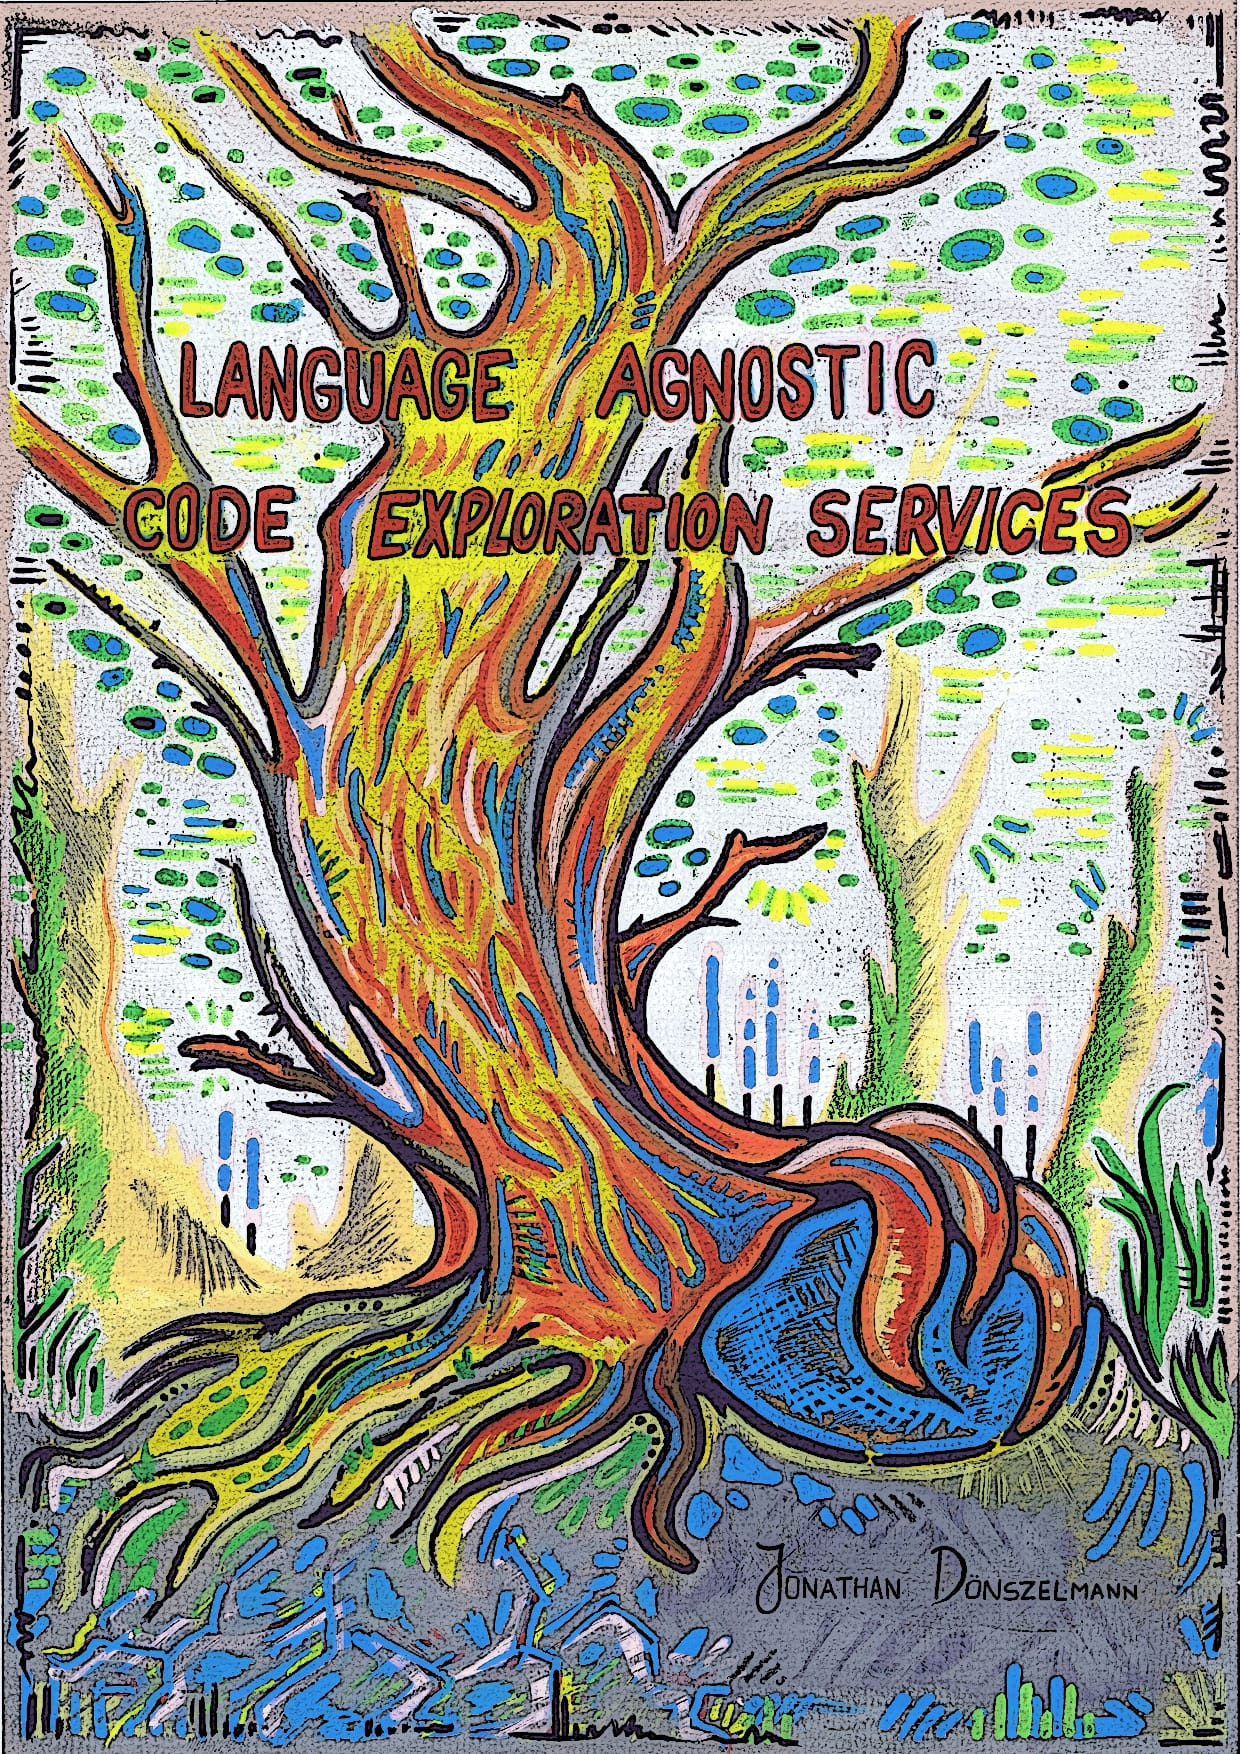
\includegraphics[width=\paperwidth,height=\paperheight]{../images/cover}%
        };
    \end{tikzpicture}
    \cleardoublepage{}
    \makeformaltitlepages{% !TEX root = document.tex

Programmers spend significantly more time trying to comprehend existing code than writing new code.
They gain an understanding of the code by navigating the code base in an IDE, by reading documentation online, and by browsing code repositories on websites such as GitHub.
Creating rich experiences for a variety of programming languages across those various media is a large effort.
This effort might be worthwhile for popular languages, but for niche or experimental languages the required effort is often too large.
Solutions to reduce this effort in IDEs exist, like LSP, but to reduce the effort in other places, we introduce the \emph{Codex metadata format}, separating the language-specific generation of code metadata from its language-agnostic presentation.
We demonstrate this approach by implementing five language-specific generators (from LSP, CTAGS, TextMate, Agda and Elaine) and two language-agnostic presentations (PDF documents, and a code viewer website) of code and metadata.
To demonstrate different kinds of code metadata, we implemented four different code exploration services: syntax coloring, code navigation, structure outline, and diagnostic messages.
As part of this thesis, we submitted a paper in which we demonstrate that the Codex format successfully decouples languages and their metadata from their presentations.
In this thesis, we continue the work from that paper, discussing each topic more in-depth and expanding on ideas from the paper.
}

    % !TEX root = document.tex

\chapter*{\label{chap:Preface}Preface}
\addcontentsline{toc}{subsection}{Preface}
%
%\begin{figure}[h!]
%   \centering
%   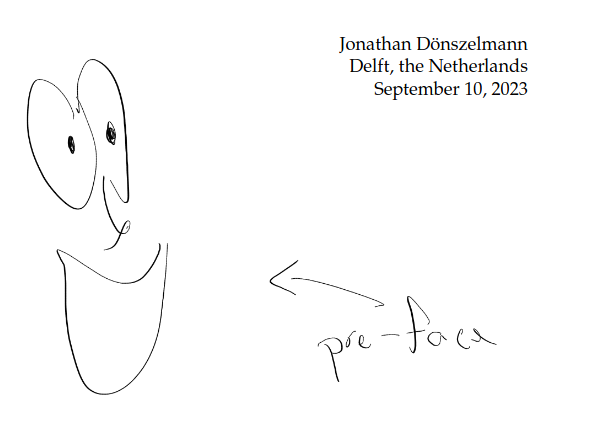
\includegraphics[width=0.5\textwidth]{../images/original-preface}
%   \caption{Original Preface by Terts Diepraam}
%   \label{fig:original-preface}
%\end{figure}


\vspace{1cm}
\begin{flushright}
\theauthor{}\\
Delft, the Netherlands\\
\today{}\\
\end{flushright}


    \cleardoublepage\tableofcontents
%\cleardoublepage\listoffigures
%\cleardoublepage\listoftables
    \cleardoublepage\mainmatter{}

    \newtheorem{definition}{Definition}

    % !TEX root = document.tex

\chapter{\label{chap:introduction}Introduction}

Introduction here.
    % !TEX root = document.tex


\chapter{Editor Services}
\label{chap:editor-services}

Although programmers may have started out manually punching their programs into punchcards,
or even changing the wiring of the computer just to program it, few people still do this nowadays.
Instead, programmers write computer programs for a computer, on a computer.
The obvious advantage of that is of course that it is much easier to change the program after
it was written the first time.

Early on, there was \texttt{ed}~\autocite{ed}, short for `editor'.
\texttt{ed} was one of the standard tools included on all unix operating systems, and can still be used on many modern computers.
However, it has also been called ``the most user-hostile editor ever created'' (by Peter H. Salus) because of the
minimal visual feedback it gives.
For all kinds of different errors, \texttt{ed} simply prints a \texttt{?} without further context.

Since then, a lot has changed, and editors have become significantly more advanced.
Not just by actually allowing users to see the document they are editing, a feature which \texttt{ed} notably lacked,
but also by actively helping programmers to write their program.
For example, colouring different parts of a program based on their syntactical meaning, and completing words and lines based on context.
To provide these features, te editor will have a certain amount of knowledge about the language that is being edited, such as the language's grammar.

However, some editors know a lot more about the language that is being written than just the grammar.
A modern \ac{IDE} may know about different libraries you might want to use and their documentation,
work for multiple programming languages in large projects, and even automatically generate whole pieces of code based on context.
As well as simplifying writing code, an \ac{IDE} can also help with compiling and running code, as well as provide tooling to interactively debug it.
All these tools, which make it easier to write code, are called editor services, a term coined by \textcite{KatsKV08}

\section{An overview of editor services}\label{sec:an-overview-of-editor-services}

Different editors provide different editor services.
Nevertheless, the kinds of services provided overlap significantly, meaning we can try to list the main classes of services.
In ``The State of the Art in Language Workbenches'',~\autocite{ErdwegSV13} provides a feature model of language workbenches
\footnote{More will be said about language workbenches in ...}.
When \citeauthor{Fowler2004} first wrote about language workbenches, the relation between language workbenches and \acp{IDE} was already discussed~\autocite{Fowler2004}.
Hence, the feature model by \citeauthor{ErdwegSV13} also describes editor services as one of six main features of a language workbench.
In the feature model, editor services are further subdivided into

\begin{itemize}
    \item Syntactic services
    \begin{itemize}
        \item Highlighting
        \item Outline
        \item Folding
        \item Syntactic completion
        \item Diff
        \item Auto formatting
    \end{itemize}
    \item Semantic services
    \begin{itemize}
        \item Reference resolution
        \item Semantic completion
        \item Refactoring
        \item Error marking
        \item Quick fixes
        \item Origin tracking
        \item Live translation
    \end{itemize}
\end{itemize}

The feature model by \citeauthor{ErdwegSV13} was adapted by \citeauthor{Pelsmaeker2018} into a list of just editor services~\autocite{Pelsmaeker2018}.
This derived list further splits the services into more categories, as well as renaming a few to sound more intuitive.
For example, syntax highlighting was renamed to syntax colouring as highlighting would imply a change in background colour.
We also annotated each service in this list with a short explanation, not present in the original list by \citeauthor{Pelsmaeker2018}:

\begin{itemize}
%    \setlength\itemsep{-1em}
    \item Editor:
    \begin{itemize}
%        \vspace{-2\topsep}
%        \setlength\itemsep{-0.3em}
        \item Syntax colouring: giving different colours to different syntactical elements
        \item Code folding: hiding blocks of related code to reduce visual clutter
        \item Code completion: suggesting word and line completions based on context
    \end{itemize}
    \item Navigation and structure:
    \begin{itemize}
%        \vspace{-2\topsep}
%        \setlength\itemsep{-0.3em}
        \item Structure outline: visualizing the structure of code to quickly navigate it
        \item Reference resolution: providing quick navigating between related code
    \end{itemize}
    \item Help and documentation:
    \begin{itemize}
%        \vspace{-2\topsep}
%        \setlength\itemsep{-0.3em}
        \item Documentation: showing documentation of written elements in-editor
        \item Signature help: showing previews of an items parameters after typing the item
    \end{itemize}
    \item Actions and transformations:
    \begin{itemize}
%        \vspace{-2\topsep}
%        \setlength\itemsep{-0.3em}
        \item Automatic formatting: rewriting source code based on certain formatting rules
        \item Rename refactoring: language and context aware search-and-replace.
              May sometimes be called structural search and replace~\autocite{jetbrains_ssr}.
        \item Code actions: language specific actions that typically fix or transform code~\autocite{lsp_code_actions}
    \end{itemize}
    \item Life cycle
    \begin{itemize}
%        \vspace{-2\topsep}
%        \setlength\itemsep{-0.3em}
        \item Diagnostic messages: showing warnings and errors in the source text
        \item Debugging: stepping through code as it runs, allowing inspection of variables
        \item Testing: running tests directly from the editor, showing their success or failure
    \end{itemize}
\end{itemize}

\section{Providing editor services}\label{sec:providing-editor-services}

To provide editor services, the editor needs some information about the language it is providing services for.
The amount of information, depends on what services are provided.
The way these features are provided differs per language and editor.

\todo{
    if relevant, provide an example of for example how rust-analyzer and maybe another editor service provide do this.
    In any case mention how in many cases, editor services sort of integrate with a compiler since some services you want in an editor are also those you want in a compiler
    Also talk about editor services being dynamic
}


\section{Porting editor services}\label{sec:porting-editor-services}

Because editors need knowledge about a language to provide editor services for that language, not even the most advanced editor will support all languages.
Especially \acp{DSL} often have very little native support.
That is why many editors provide a way to be extended by users, often in the form of a plugin system.
That way, when a new language is created, users can add support for that language to the editor instead of the authors of the editor.

This leads to a complicated problem, called the \ac{IDE} portability problem~\autocite{KeidelPE16}.
The way every editor provides editor services is slightly different.
This means that supporting $m$ languages in $n$ editors requires $m \times n$ editor plugins, one for each
combination of a language and editor.

The $m \times n$ problem often becomes an issue of responsibility.
Creators of editors do not want to be responsible for supporting every language.
On the flip side, language authors can't always support every editor there is.

In ``Portable Editor Services'', Pelsmaeker~\autocite*{Pelsmaeker2018} investigates this issue, and proposes a solution: \ac{AESI}.
\ac{AESI} is a system to create editor plugins.
\todo{Briefly explain AESI, then talk about LSP itself trying to solve the problem, and language workbenches which generate editor services based on a language's definition}


\section{Language Servers}\label{sec:language-servers}
    % !TEX root = document.tex

\chapter{Code Exploration Services}
\label{chap:code-exploration-services}

As the name implies, a programmer's job generally involves writing programs.
However, a vital part of writing code is also reading and exploring code.
In the book ``Clean Code: A Handbook of Agile Software Craftsmanship''~\autocite{martin_reading_code_ratio},
the author estimates that a programmer may spend up to ten hours reading code for every hour of time they spend writing code.

Some examples of such tasks that do not necessarily involve writing code might be reading code from last week, or code written by colleagues.
Especially in teams, programmers also commonly review code, which mainly involves reading code and verifying its correctness.
Furthermore, programmers may read code on websites such as \url{https://stackoverflow.com} and \url{https://github.com},
and in documentation, to learn from others about how to solve a problem.
All these interactions programmers might have with code, that do not involve writing code, we will call code exploration from now on.

% Reference https://www.informit.com/articles/article.aspx?p=1235624&seqNum=5?
% Reference https://www.youtube.com/watch?v=QoZU2yN8caY

Exploring programs in an editor can be easier than in other places, because many editors provide editor services that simplify exploring and understanding code.
Still, editors aren't the only places where programmers explore code.
The main other locations being on websites, in PDFs (for example, a paper), and in books.
Although these places are used for exploring code, they often provide few services that help programmers to do so like editors would.
It might be that only syntax colouring is available, for example.
However, we think that those services traditionally found in editors, might actually be useful when reading code in other places besides editors
Those services, which are useful outside an editor, we call code exploration services.

As an example, and a notable exception to websites only providing syntax colouring, there is Github\footnote{\url{https://github.com}}.
GitHub, apart from being a git server where programmers store their code, is also a place where lots of code is read.
For example, as a part of code reviews.
To aid programmers, GitHub has been getting more and more features that make exploring code simpler such
as more advanced search functionality, and recently code navigation.
The latter is only supported for a few specific programming languages though\footnote{\url{https://docs.github.com/en/repositories/working-with-files/using-files/navigating-code-on-github}}.

This does raise the question: what other services might (in general) be useful code exploration services?

\section{An overview of code exploration services}\label{sec:an-overview-of-code-exploration-services}

In chapter~\ref{chap:editor-services}, we discuss a list of important editor services.
For each, we will discuss whether they might be useful as code exploration services as well.
Before we can do that however, we first need to discuss when a code exploration service is useful.
We think that a code exploration service is useful, if it has the potential to help a programmer understand the program they are reading quicker.
With that definition, how useful is each the editor services as code exploration services?

\subsection*{Syntax colouring}

The usefulness of syntax colouring for code comprehension has been extensively researched.
Although one study, with a low sample size, seems to claim that colouring has a positive effect for novices, but not for
more experienced programmers~\autocite{Sarkar15a-0}, there is also work that concludes that the effect is in fact minimal.
In a study where eye movements of participants were tracked, no significant difference between black-and-white code and coloured code\autocite{beelders2016syntax}.
Similarly, novice students would not perform better at programming tasks where syntax was coloured compared to tasks where syntax was not coloured~\autocite{HannebauerHG18}.

Although there seems to be relatively little evidence that syntax colouring actually helps programmers, it is what many programmers will expect when reading code.
All editors evaluated by \citeauthor{Pelsmaeker2018} support syntax colouring to a certain extent~\autocite{Pelsmaeker2018},
and one could argue that the coloured text distinguishes code from the surrounding content.
Therefore, we would argue that syntax colouring can be useful when exploring code.

\todo{do I want full cited explanations of each of this lke above, or is that not really important for the research on file formats and should I just state that
these are the things we're going to look at}
\subsection*{Code folding}

\subsection*{Code completion}

Code completion only helps programmers write code, and has little to do with code exploration.

\subsection*{Structure outline}

\subsection*{Reference resolution}

\subsection*{Documentation}

\subsection*{Signature help}

\subsection*{Automatic formatting}

\subsection*{Rename refactoring}

\subsection*{Code actions}

\subsection*{Diagnostic messages}

\subsection*{Debugging}



\subsection*{Testing}

%As demonstrated by Github, it certainly seems like it is possible to provide more services to the readers of programs.
%One might call such services for code readers, code exploration services.
%However, that's not quite

\subsection{Code search}\label{subsec:code-search}

Although the list of code exploration services has its roots in a list of editor services, which itself has its roots in
frequently cited theory by \citeauthor{ErdwegSV13}, we actually think that one feature may be missing from the original list.
That feature is search.
That search is missing is interesting, because the feature is pretty much universally supported by editors, even `dumb' ones.
Even many websites, where we showed that often relatively few services are supported, offer advanced search options.

So why is search missing?


\section{Availability of code exploration services}\label{sec:availability-of-code-exploration-services}

\todo{Survey of other websites, showing that they pretty much only support syntax colouring}



\subsection{Github}



\subsection{Gitlab}
\subsection{MdBook}
\subsection{StackOverflow}
\subsection{Reddit}
\subsection{Latex and PDF}
\subsection{Bootlin}
\subsection{Monaco}


%However, to take advantage of editor services, a programmer needs to download the sourcecode to their own computer and actually
%open the program in an editor, which can be inconvenient.

% Sometimes you look at code not in an IDE (like online, or in papers)
% What services are available in those places?
% Most places provide syntax colouring
% Some places provide code navigation (Github, cross referencers)
% However for very limited cases (only some languages)
% What's different from IDEs to these places where code is read? Well,
% What services could theoretically be provided?
% We call these services code exploration services


%jupyter
%mdbook
    % !TEX root = document.tex

\chapter{Designing Codex}
\label{chap:designing-codex}

In the previous chapter,~\cref{chap:code-exploration-services},
we concluded that there exists a problem analogous to the IDE portability problem with existing systems that provide code exploration services.
All such existing systems are narrow in scope.
We called this problem the \problem{\times} problem for code exploration services.
In this chapter we will design a prototype system we call the Codex that aims to solve this problem by being less narrow in scope.

Note that Codex is the name of the entire prototype we design, as well as the name for the metadata format used by the prototype.
We will always refer to the \emph{Codex metadata format} explicitly when we refer to the format rather than the prototype in its entirety.

In order for Codex to be less narrow in scope than existing solutions,
Codex will have to support both multiple code exploration media, as well as multiple programming languages.
To do this while avoiding the \problem{\times} problem for code exploration services, Codex needs to consist of two kinds of components:
language-specific systems that can provide information about a program written in a specific language,
and language agnostic systems that can create code exploration services from this information.
Any pair of such systems should be able to work together, to make the complexity \problem{+}.
We will call the language-specific systems Codex metadata generators, or metadata generators for short,
and we call the language-agnostic systems presentation generators.

\section{Code Exploration in Static Media}\label{sec:code-exploration-in-static-media}

Comparing this to \ac{LSP}, metadata generators are analogous to language servers, with presentation generators taking the role of editors.
Note that we were careful to say that presentation generators take the role of an editor, presentations themselves do not.
Although we explore code through some kind of presentation of the code in a medium, together with editor services,
many media have important restrictions on what we can do in them.

Take PDF documents as an example.
While an editor can dynamically make requests to a language server running in the background to get up-to-date information about the program which is written,
we cannot make requests like that inside a PDF document.
We illustrate this in figure \cref{fig:static-vs-dynamic}.

Instead, if we want to provide code exploration services in a PDF document, those need to be embedded into the PDF itself at the moment the PDF is generated.
This baking-in process may involve colouring some text in the document, notably the parts where source code is presented,
and, for example, adding extra hyperlinks to navigate between different pieces of source code.
This embedding is done by the presentation generator, making \emph{it} analogous to an editor with the capability to access language-specific metadata.
In that way, the presentation generated by the presentation generator has the possibility to be entirely static.

\begin{figure}
    \centering
    \begin{tikzpicture}[font={\xkcd}]

        \begin{pgflowlevelscope}{\pgftransformscale{3}}
            \draw (0.75,1.333) node {\faUser};
        \end{pgflowlevelscope}

        \draw[-stealth, ultra thick, draw={rgb:red,128;green,29;blue,39}](3,4) -- (4,4);
        \draw (3.5,4.5) node {Uses};

        \node [draw, thick, shape=rectangle, minimum width=2cm, minimum height=2cm, anchor=center] at (5,4) {};
        \draw (5,4.25) node {PDF};
        \draw (5,3.75) node {Document};

        \draw (7.5,5.5) node {Can't};
        \draw (7.5,5) node {make};
        \draw (7.5,4.5) node {requests};
        \draw[-stealth, ultra thick, draw={rgb:red,128;green,29;blue,39}](6,4) -- (9,4);

        \begin{pgflowlevelscope}{\pgftransformscale{2}}
            \draw (3.75, 2) node {\faTimes};
        \end{pgflowlevelscope}

        %%%%%%%%%%%%%%%%%%%%%%%%%%%

        \begin{pgflowlevelscope}{\pgftransformscale{3}}
            \draw (0.75,2.666) node {\faUser};
        \end{pgflowlevelscope}

        \draw (3.5,8.5) node {Uses};
        \draw[-stealth, ultra thick, draw={rgb:red,128;green,29;blue,39}](3,8) -- (4,8);

        \node[draw, thick, shape=rectangle, minimum width=2cm, minimum height=2cm, anchor=center] at (5,8) {};
        \draw (5,8) node {Editor};

        \draw[-stealth, ultra thick, draw={rgb:red,128;green,29;blue,39}](6,8) -- (9,8);
        \draw (7.5,9) node {Requests};
        \draw (7.5,8.5) node {from};

        \node[draw, thick, shape=rectangle, minimum width=2cm, minimum height=2cm, anchor=center] at (10,8) {};
        \draw (10,8.25) node {Language};
        \draw (10,7.75) node {Server};


        %%%%%%%%%%%%%%%%%%%%%%%%%%%
        \begin{pgflowlevelscope}{\pgftransformscale{3}}
            \draw (0.75,0) node {\faUser};
        \end{pgflowlevelscope}

        \draw[-stealth, ultra thick, draw={rgb:red,128;green,29;blue,39}](3,0) -- (4,0);
        \draw (3.5,0.5) node {Uses};

        \node [draw, thick, shape=rectangle, minimum width=2cm, minimum height=2cm, anchor=center] at (5,0) {};
        \draw (5,0.25) node {PDF};
        \draw (5,-0.25) node {Document};

        \draw (7.5,1) node {Generates};
        \draw (7.5,0.5) node {PDF};
        \draw[stealth-, ultra thick, draw={rgb:red,128;green,29;blue,39}](6,0) -- (9,0);

        \node[draw, thick, shape=rectangle, minimum width=2cm, minimum height=2cm, anchor=center] at (10,0) {};
        \draw (10,0.5) node {Language};
        \draw (10,0) node {Agnostic};
        \draw (10,-0.5) node {Tool};

        \draw (12.5,1.0) node {Generates};
        \draw (12.5,0.5) node {Metadata};
        \draw[stealth-, ultra thick, draw={rgb:red,128;green,29;blue,39}](11,0) -- (14,0);

        \node[draw, thick, shape=rectangle, minimum width=2cm, minimum height=2cm, anchor=center] at (15,0) {};
        \draw (15,0.5) node {Language};
        \draw (15,0) node {Specific};
        \draw (15,-0.5) node {Tool};

    \end{tikzpicture}

    \caption{
        Although a language-agnostic editor can directly make requests to a language-specific source of information (as is the case with \ac{LSP}),
        this architecture cannot work in code exploration media where making requests are impossible such as in PDF documents.
        Code Exploration Services must instead be embedded in such media whenever they are generated.
    }
    \label{fig:static-vs-dynamic}
\end{figure}

\section{Making Metadata Language-Agnostic}\label{sec:making-metadata-language-agnostic}

Between metadata generators and presentation generators, information needs to be exchanged to enable code exploration services.
This information is metadata, information \emph{about} a program which is analysed.
For example, this metadata may be information about which parts of a program references which other parts of a program to facilitate code navigation.

It is important that the way this metadata is stored is in no way tied to any specific programming language.
If that were the case, we are unnecessarily limiting the scope of Codex, just like the narrow tools we discussed in~\cref{sec:code-exploration-services-in-other-media}.
Despite the success of \ac{LSP}, \ac{LSP} too made this mistake.
In \ac{LSP}, a symbol can fall into one of a limited set of categories, which is the symbol's \texttt{SymbolKind}~\autocite{lsp_symbol_kind}.

It is not difficult to find languages with symbol kinds that do not fit into these limited number of categories: Rust has structs but a struct is not a valid \texttt{SymbolKind}, and Haskell's typeclasses fail to fit in as well.
Although substitutes could be used, a struct might become a class, and a typeclass an interface, this does not always work.
C++ has both classes and structs, should these both be labelled as classes in \ac{LSP}?

The approach \ac{LSP} takes, with a limited number of categories into which all languages must fit is doomed to fail.
Because of the wide variety of programming languages in existence, and subtle differences in meaning of language constructs between languages,
we cannot make an exhaustive list of syntactical categories which applies to every language there is.

\subsection{Hierarchical Categorisation}\label{subsec:hierarchical-categorisation}

An approach that avoids making such an exhaustive list was first used for TextMate, an editor for MacOS~\autocite{textmate}.
This approach is now used in facilitating syntax highlighters in multiple editors, also Visual Studio Code.

TextMate uses custom syntax specifications of languages in the form of regular-expression based grammars in order to support syntax colouring.
Such grammars would give different syntactical elements a label.
Colour themes could then apply different colours to items with different labels.
Because the people who make grammars were not necessarily the same as the people making the themes,
a standardised labelling system had to be invented such that all themes could be compatible with all grammars.

Instead of making an exhaustive list, TextMate uses a hierarchical approach, which is not so different from taxonomies in biology.
In TextMate, an \texttt{=} in a variable assignment in Rust might be labelled \texttt{keyword.operator.assignment.rust}.
The dots in this label separate parts of the label, going from generic to specific.
First of all, the \texttt{=} is a keyword, but more specifically an operator, specifically meant for assignment, specifically in Rust.

Now, TextMate themes can match on these labels in a similar way to how CSS classes match:
if a theme only knows how to colour keywords, this assignment operator gets the same colour as all keywords.
However, a theme can also specify a specific colour for all \texttt{keyword.operator}s, or even more specific.
The advantage is that this system can both capture all the language-specific details of syntax,
as well as being easy to read for tools which might not be aware of these language-specific details.

In the Codex metadata format, to be completely language-agnostic,
it makes sense to make any language-specific labelling such as syntactical categories hierarchical.

\section{Generating All Metadata At The Same Time}\label{sec:generating-all-metadata-at-the-same-time}

\ac{LSP} is usually Lazy.
Only when an editor needs information for editor services, it makes a request to the Language Server for it.
In contrast, presentation generators generate a presentation of all the source code at the same time,
embedding code exploration services into the medium.
This process needs access to \emph{all} metadata at the same time.

Thus, a request-response model like \ac{LSP} makes little design for communication between metadata generators and presentation generators.
Instead, a more instantaneous method of communication can be used: a data format instead of a protocol.
This has several advantages.


%vendor lock-in
%some langs can't get static analysis


    % !TEX root = document.tex


\chapter{The Codex Metadata Format}
\label{chap:codex}

In the previous chapter,~\cref{chap:code-exploration-services}, we concluded that there exists a problem with current
systems that provide code exploration services just like there is the IDE portability problem for editor services.
We called this problem the \problem{\times} problem for code exploration services.
In this chapter we will design a prototype system we call Codex that solves this problem.
First we will more precisely define the goals of Codex, after which we will outline our approach which we will then demonstrate.

\section{The Goal of Codex}\label{sec:the-goal-of-codex}

%Codex transforms the \problem{\times} problem into a \problem{+} problem in a similar fashion to how \ac{LSP} transforms the IDE portability problem.

In an editor, source code is constantly changed, which means that any information needed for editor services must constantly be recalculated based on new changes to the source code.
With \ac{LSP}, these recalculations happen in the language-specific `language server', with which the editor must continually communicate.
Such recalculations are not always possible in other code exploration media.
To demonstrate Codex, we will focus specifically on two media in this chapter and thesis: HTML webpages and PDF documents generated through LaTeX.

Neither of these media easily support the constant recalculation we see with editor services for different reasons.

In PDF documents the reason is simple, you cannot easily execute any code in PDFs if at all.
Furthermore, when PDF documents are printed, all interactivity is certainly lost while the possibility of providing code exploration services like syntax colouring is not.
Instead, we would like to ``bake in'' the code exploration services the moment the PDF is generated by, for example colouring text, inserting hyperlinks and adding hover text.
We illustrate this in~\cref{fig:static-vs-dynamic}.

%\section{A static Language Server Protocol}\label{sec:a-static-language-server-protocol}

% Take PDF documents for example.
% Because it is near impossible to run code in PDF documents, we cannot make requests to language-specific tools like a language server.
% Instead, if we want to provide code exploration services in PDFs, we would like to essentially bake them in at the moment the PDF is generated by colouring text, inserting hyperlinks and adding hover text.

%Any information needed to provide code exploration services in a PDF is static, which means that there is no reason to request such information on-demand.
%This is true for all code exploration services: the code they provide services for does not change, by definition.

%That means that a medium with code exploration services could even bake-in the code exploration services by, for example, colouring text, inserting hyperlinks and adding hover text.

% We illustrate the difference between how an editor gathers information for editor services using \ac{LSP}, and how in \cref{fig:static-vs-dynamic}.
% In that figure, \ac{LSP} solves the
%
% We call tool that creates code presentations with baked-in code exploration services, a presentation generator, or generator for short.
% Generators are medium-specific: one generator could create PDF documents and another webpages.
% Then, to avoid the \problem{\times} problem, generators should be language agnostic and talk over a standardised interface to language-specific tools.



On Websites, interactivity is not as impossible as in PDF documents, and there are examples of web-based editors which communicate with an LSP over the internet~\autocite{che, theia}.
However, these web-editors only do that because they allow users to change code requiring constant updates.
For providing only code exploration on static webpages, the overhead is both undesired and unnecessary.
Undesired because it makes exploring code slower and unnecessary because just like with PDFs the code exploration services can be baked in to the page.

Thus goal of Codex is to show that we can support code exploration services in different media, in a language-agnostic way, while avoiding the \problem{\times} problem.
To demonstrate this two goal, we first use metadata in the Codex format to provide rich code exploration on websites and PDF documents.
Then, we show two approaches to gather metadata from code bases: adapting existing tools made to support existing languages; and to directly gathering metadata from a parser and type checker of a \ac{DSL}.
This shows how the Codex format is useful to present code for small programming languages for which no custom tooling is available.



%Although we cannot say that LSP solved the IDE portability problem, the project has considerably improved the status quo.
%Using LSP, many editors and languages can communicate.
%However, because the \ac{LSP} has a client-server architecture it is hard to
%
%To show that a metadata format can indeed power code exploration services, we have created a proof-of-concept\footnote{The source code for this proof of concept can be found on GitHub at \url{https://github.com/url-anonymized}}.
%The goal of this proof of concept is twofold:
%to demonstrate that it is feasible to use statically generated metadata to provide code exploration services in various media;
%and to show that by using a data format like ours, we can decouple the production and consumption of such static metadata in a language-agnostic way.
%
\todo{figure commented below}
\begin{figure*}[ht]
    \centering
    \begin{subfigure}[b]{0.49\textwidth}
        \centering
        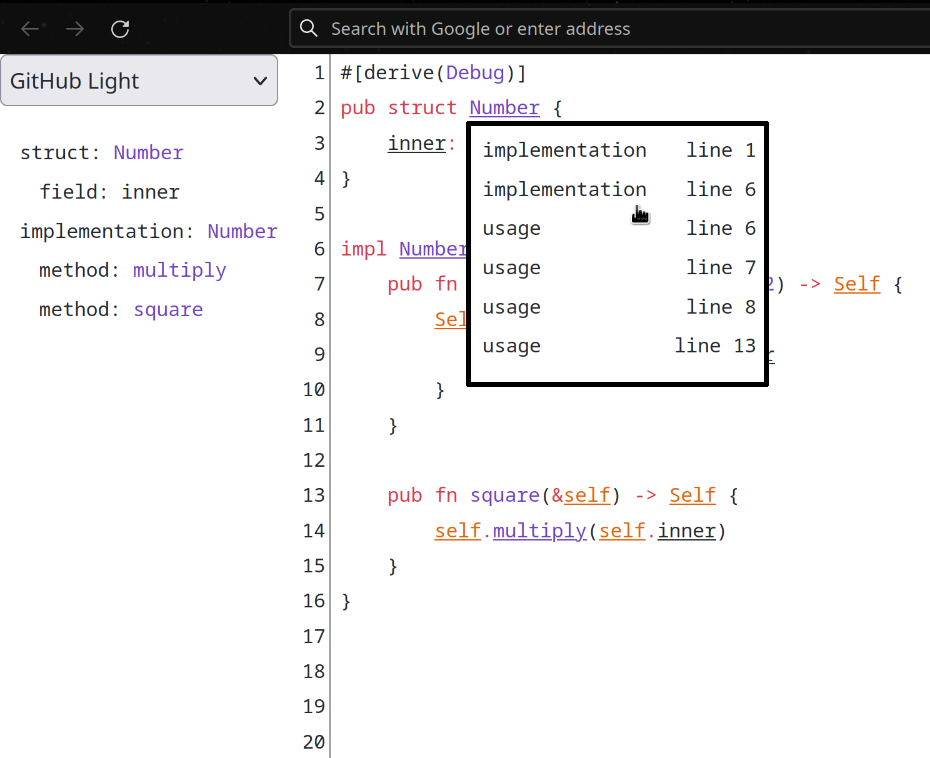
\includegraphics[width=\textwidth]{../images/codex-html}
        \caption{
            A fragment of Rust code presented in an interactive HTML webpage.
            The color information, reference information (underlines), outline, and warnings are derived from metadata stored in the Codex format.
            When a declaration in the code is referenced more than once, hovering over the underlined name opens a pop-up listing all its usages.
            Clicking one of the usages in the list instantly jumps the PDF viewer to the relevant code.
        }%
        \label{fig:demo.html}
    \end{subfigure}
    \hfill
    \begin{subfigure}[b]{0.49\textwidth}
        \centering
        \codeNumberRs
        \caption{
            The same fragment of Rust code as shown in \cref{fig:demo.html},
            but embedded in this paper through LaTeX source code generated from the Codex metadata format.
            When this paper's \acs{PDF} is viewed digitally, underlined elements are clickable and navigate to the referenced location.
            When an item is referenced more than once, superscript annotations are inserted that facilitate navigation. \\
        }%
        \label{fig:demo.latex}
    \end{subfigure}
    \caption{A demonstration of our proof of concept, presenting source code on a website and in this document.}
    \label{fig:demo}
\end{figure*}

% \paragraph{Reading this Section}
%
% In this section, we demonstrate a proof of concept of Codex.
% Part of this demonstration consists of examples of codex converting source code to LaTeX, which we display as part of this document.
% This entire section is written in a way that, when printed in black-and-white, it is readable.
% However, some parts of the demonstration will contain color, and interactive elements which will not be visible in black-and-white.
% Each example does have an explanation of what could be visible when read in color or digitally.


\section{Presenting Code on Websites through HTML}
\label{sec:demonstration.html}

HTML is a standard format for documents designed to be displayed in web browsers.
Together with CSS and JavaScript, HTML can be used to create websites with complex graphical user interfaces and visualizations.
Many websites such as StackOverflow, GitHub and GitLab can visualize users' source code, sometimes with some basic code exploration services.

In our demonstration we can produce HTML documents from source code and its corresponding Codex metadata.
A screenshot of the resulting website is shown in~\cref{fig:demo.html}.

In the generated HTML document, we implemented several code exploration services:
syntax coloring, structure outline, code navigation, and diagnostic messages.
Code navigation is implemented by adding hyperlinks to the code, though when more than one reference exists, a pop-up is shown when hovering over underlined items, allowing users to choose where to navigate.
Diagnostic messages are shown by underlining an item in yellow, which when hovered over shows the associated compiler warnings and errors.

% To generate these documents, we take the metadata, and use it to tokenize the source text.
% Tokens are spans of text which have the same metadata.
% Because the metadata is based on the syntactical structure of the code, these tokens usually correspond with syntactical elements.

% \todo[inline]{remove this}
% Then we wrap each token in HTML \texttt{span} elements, with the correct CSS classes determined based on the metadata to color each token.
% Here, we also insert link information.
% Tokens are annotated with unique identifiers that allow a JavaScript \texttt{onclick} handler to navigate the code.
% These identifiers are also used to navigate from outline items to source code.
% The outline itself is generated separately, but also uses the tokenization to highlight the pieces of code embedded in the outline.

It is possible for users to change the theme of the HTML visualization.
Instead of assigning colors to tokens, we add CSS classes based on the token's classification (See \cref{sec:demonstration.generating.textmate} for more details).
At the same time, multiple TextMate syntax theme definitions are translated to CSS and included with the HTML document.
Users can choose which CSS rules are applied by choosing a theme in the top left.


\section{Presenting Code in PDF Documents through LaTeX}
\label{sec:demonstration.latex}

A different presentation of the same Rust code of~\cref{fig:demo.html} is shown in~\cref{fig:demo.latex} embedded into this paper's text through generated LaTeX code.
Just like with HTML, the Codex proof of concept can also generate LaTeX source code based on metadata in the Codex format.
The two visualizations are adjusted to their medium, but both rely on the Codex metadata format.

% And yet, some elements are similar. Syntax is still colored (using~\texttt{xcolor}), although now with a static theme which readers cannot change.
% Underlined elements are links (using~\texttt{hyperref}), and there is a possibility to generate a digital outline in the resulting PDF document resulting from the LaTeX source.
% We have not included an outline of the code in this paper, since we think it would be distracting in this context.

One extra aspect of our LaTeX generator is that it can generate LaTeX for multiple files from the same project, if the metadata contains that information.
\Cref{fig:demo.latex.reference} shows source code from a different file in the same Rust project as the example in \cref{fig:demo}.
The two files reference each other, and when viewing this paper digitally, hyperlinks enable quick navigation between the two figures.

When there are multiple references, instead of providing a drop-down menu as shown in the generated website, in the PDF we add multiple links in superscript to parts of the code that reference multiple other locations in the code.
An example of this can found in \cref{fig:demo.latex}, \cref{fig:demo.latex.reference}, and \cref{fig:elaine}.

Because both the HTML presentation and this LaTeX presentation rely solely on metadata in the Codex format,
both are completely language-agnostic.
Although \cref{fig:codex-json-metadata} is mainly meant to demonstrate what the Codex metadata format looks like when it is serialized, the syntax coloring in the example itself is created using Codex.
Therefore, \cref{fig:codex-json-metadata} is also a demonstration of how, through the Codex metadata format, we can present code written in different languages.

% In this section, we demonstrate a proof of concept of Codex.
% Part of this demonstration consists of examples of codex converting source code to LaTeX, which we display as part of this document.
% This entire section is written in a way that, when printed in black-and-white, it is readable.
% However, some parts of the demonstration will contain color, and interactive elements which will not be visible in black-and-white.
% Each example does have an explanation of what could be visible when read in color or digitally.


\section{Generating Metadata from Existing Tools}

Codex metadata can be generated either directly by instrumenting compilers, or by adapting independently developed tools.
In this section, we show how we used several of such existing tools to generate metadata and how we converted this metadata into the Codex format.

\paragraph{TextMate Grammars}
\label{sec:demonstration.generating.textmate}

The first tool that we use to generate Codex metadata are grammar definitions.
A common standard for grammar definitions supported by code editors is the one originally used by the TextMate editor~\cite{textmate}.
Grammar definitions for many languages, both small and large, are freely available online, mostly with the purpose to be used in editors.
Almost all editors either have native support for these TextMate grammar files, or have plugins which add this support.

TextMate grammars are not full context-free grammars, but instead function by applying regular expressions to fragments of source code.
Based on which regular expressions matched words in the code, other regular expressions are brought in and out of scope to allow moderately complex syntaxes to be parsed.
Due to their design, TextMate grammars quite often perform well even in the presence of syntax errors.

TextMate introduces a way to hierarchically classify tokens based on the token's function in a programming language.
We discussed in \cref{sec:demonstration.format} how we use this function for syntax coloring and other code exploration services in the Codex format.
Because we use this system for syntax coloring, translating from TextMate output to the Codex format is very simple.
TextMate grammar files contain such classifiers, and we can put those directly into the Codex format.

% We use this hierarchical classification for syntax coloring, but also for other parts of metadata that need categorization.
% We discussed this in depth in \cref{sec:demonstration.format}, but the inspiration to use classifications in metadata came from TextMate.
% This also means that translating from a TextMate parser to the Codex format is very simple.
% TextMate grammars already contain classifications.

% \todo[inline]{Already explained}

% In Codex, TextMate grammars can be associated with a certain programming language.
% When Codex analyses a file of that programming language, and a grammar is available for that language, Codex uses the grammar to categorize the tokens in the file.

% In \cref{fig:codex-json-metadata}, we can see an example of this.
% We see that a token at offset $4$ with a length of $4$ has the syntax category \texttt{keyword.declaration.enum.rust}.
% This corresponds with the code in \cref{fig:codex-field}, where after $4$ characters, there is the keyword \texttt{enum}, which is $4$ characters long.
% The dots in this category separate hierarchical levels; after every dot, the category becomes more specific.
% Based on that category, the token is colored red in \cref{fig:codex-field} by the theme we used.

Previous parsers using TextMate (like the one for VS Code and TextMate itself) are designed to work in combination with an editor.
These proved hard to integrate in Codex, in part because they were designed to directly output color information as opposed to token classifications.
For our proof of concept, we wrote a custom TextMate parser in Rust, which we have tested on grammar definitions of many large languages such as the ones for Rust, TypeScript, and Haskell.

\paragraph{CTAGS}
CTAGS~\cite{ctags} is a tool that can provide primitive editor services in terminal-based editors such as Vim.
To do this, CTAGS parses source files of many different languages and can generate so-called tags files from that.
Vim can then read these tags files to allow programmers to search for definitions in a code base.
CTAGS does not provide enough information to derive code navigation from its output.
However, its output can be used to generate outlines for source files, which is what Codex does.
An example of such an outline can be found in \cref{fig:demo.html}.

\paragraph{The Language Server Protocol}

In \cref{subsec:language-servers}, we already mentioned \ac{LSP}~\cite{lsp} in the context of the \problem{\times} problem.
Although \ac{LSP} is a protocol mainly meant for editors, we can use the information that \ac{LSP} can provide and extract metadata from it.
This is very different from how \ac{LSP} is normally used for editor services, requiring live communication about a user's interaction with the code base.

To accomplish this, we first start a language server on the code base we analyze.
Then we query this language server about every token in a code base, storing all responses.
We then convert the responses such that they can be stored in the Codex format, after which the language server can be stopped again.
Because of the number of queries that need to be executed, this process can be rather slow, taking up a majority of the indexing time.
However, for this demonstration, speed was not a priority.

Codex currently queries \ac{LSP} to get both reference information and diagnostic messages.
However, the LSP can provide much more than just reference information, like documentation for items, code folding points and code actions.

We have tested Codex querying an \ac{LSP}, with both Rust's and Haskell's language server implementation.
This is also how the reference metadata in \cref{fig:demo.html}, \cref{fig:demo.latex} and \cref{fig:codex-field} is generated.

\todo{figure commented below}
\begin{figure}
    \centering
    \codeBRs
    \caption{This is the continuation of the example Rust code in figure \cref{fig:demo.latex}. Code navigation enables quick navigation between the two pieces of code when reading this paper digitally.}
    \label{fig:demo.latex.reference}
\end{figure}


\section{Producing Metadata for Small Languages: Elaine}
\label{sec:elaine}%
Small programming languages, \acp{DSL} or research programming languages, often have very little tooling available.
The time it costs to make tooling, such as editor services, build systems and documentation is often not worth the time.
However, for educational purposes, and science communication, having some simple code exploration services like syntax highlighting
and code navigation could be very advantageous.

The Codex format can help with this. The visualizations of code that Codex can generate are completely language-agnostic.
That means that if the compiler or interpreter of a \ac{DSL} can output metadata in the Codex format, all code exploration services in the Codex visualizations work out of the box.

% To demonstrate this, we present Elaine.
To demonstrate this, we implemented a Codex generator for the Elaine language.
Elaine is a domain-specific language
% developed by Terts Diepraam
that explores programming using higher order effects~\cite{PoulsenR23, elaine}.
Elaine is built for research, and it has a simple type checker and interpreter written in Haskell.

We modified the Elaine parser and type checker slightly, such that it output metadata in the Codex format directly from the parser and type checker.
Implementing these modifications took less than three hours in total, and required less than $100$ extra lines of code.
The parser directly labels the syntax with similar category names as used by TextMate, without using a TextMate Grammar itself.
At the same time, the type checker outputs reference information as a replacement to queries to an \ac{LSP}.
Since the type checker needs to resolve type references anyway, outputting the results of these resolutions is not very complicated.

\todo{figure commented below}
\begin{figure}
    \centering
    \codePaperExampleElaine
    \caption{An example piece of Elaine code. Elaine is a research language that explores programming with higher order effects. Elaine's parser and type checker were slightly modified to output metadata in the Codex format, enabling syntax coloring and code navigation. }
    \label{fig:elaine}
\end{figure}


% What's interesting to note is that the Codex metadata format has no problem supporting reference resolution for effects and elaborations, a language feature not common among larger programming languages.
% When Elaine outputs metadata, elaboration references get the \texttt{label} (see \cref{fig:codex-field}) `elaboration', allowing consumers of the metadata to visualize it.

For this paper, we fed the generated metadata from Elaine into Codex, which converts the code into a LaTeX representation.
The result of this can be found in \cref{fig:elaine}.

    % !TEX root = document.tex

\chapter{Evaluation of the Codex Metadata Format}\label{chap:evaluation}

\todo[inline]{
I'm not going to talk about my own impl of code exploration services at all here.
Just about all the tradeoffs that exists, and many possible solutions.
In a next chapter, we will actually walk through the process of implementing this, and
try the different options to report on their viability.
}


\section{Keeping code and metadata in sync}
\begin{enumerate}
    \item Storing code with metadata,
    \item Hashes
\end{enumerate}

\section{Referencing locations in source files}

\section{How to lay out the information}

\subsection{Encoding}
\begin{enumerate}
    \item bytes
    \item codepoints, unicode, utf8, utf16, etc
    \item making an index
\end{enumerate}

\section{Multi-file code exploration services}

\section{Complexity of the index format}
\subsection{Ease of generation}
\subsection{Ease of interpretation}
\subsection{Integration with existing tools}
\subsection{Intermediate formats}

\section{Compression}


    % !TEX root = document.tex

\chapter{Future Work}\label{chap:future_work}

Related work here.
    % !TEX root = document.tex
\chapter{Conclusion}\label{chap:conclusion}

\todo[inline]{this is literally from the paper, so this should definitely be changed}

We presented Codex, a language-agnostic format for describing the metadata of a code base, with the purpose of providing code exploration services in different types of presentations, such as HTML websites and LaTeX documents.
The format decouples generating the metadata from its presentation, addressing  the \problem{\times} problem for code exploration services.
The format allows the code to be explored at a point later in time from when the metadata is generated, even when the specific versions of tooling that was used on the code base is no longer available.

By implementing multiple language-specific generators, we showed that the Codex metadata format can be generated from several existing narrow tools (e.g., TextMate grammars, LSP, CTAGS) for various programming languages (e.g. Rust, Haskell).
This includes generating metadata for a Domain-Specific Language (DSL), called Elaine, demonstrating that providing code exploration services for such languages without pre-existing tooling is feasible.
The code examples in the digital version of this paper are interactive, allowing the reader to navigate between code usages and definitions.
These interactive features and the syntax highlighting are generated based on the Codex metadata format, using our language-agnostic LaTeX presentation.
Additionally, we demonstrated an interactive HTML presentation that can be used to explore a code base.
We show that the Codex format successfully decouples languages and their metadata from their presentations.

    \printbibliography{}

    
\chapter*{\label{chap:acronyms}Acronyms}
\addcontentsline{toc}{chapter}{Acronyms}

% Syntax:
% \acro{<acronym>}[<short form>]{<long form>}
% \acroplural{<acronym>}[<short plural>]{<long plural>}
\begin{acronym}

    % Order manually:

    % Acronyms here
    \acro{AST}{abstract syntax tree}
    \acro{DSL}{domain-specific language}
    \acro{IDE}{integrated development environment}
    \acro{LSP}{language server protocol}
    \acro{AESI}{adaptable editor services interface}
    \acro{JSON}{JavaScript Object Notation}
    \acro{JSON-RPC}{\ac{JSON} Remote Procedure Call~\autocite{jsonrpc}}
    \acro{PDF}{Portable Document Format}
    \acro{GUI}{Graphical User Interface}
    \acro{AI}{Artificial Intelligence}
    \acro{SLE}{Software Language Engineering}
    \acro{XML}{Extensible Markup Language \todo{remove}}

\end{acronym}

% Usage:
% \ac{<acronym>} - Singular acronym, expanded on first use, e.g. "API".
% \acp{<acronym>} - Plural acronym, e.g. "APIs"
% \acf{<acronym>} - Expanded form, e.g. "application programming interface (API)".
% \acfp{<acronym>} - Expanded form plural.
% \acs{<acronym>} - Short form, e.g. "API"
% \acsp{<acronym>} - Short form plural.
% \acl{<acronym>} - Long form, e.g. "application programming interface"
% \aclp{<acronym>} - Long form pluralaphical User Interface (GUI.
% \acsu{<acronym>} - Short form, and marks it as used
% \aclu{<acronym>} - Long form, and marks it as used

% \acresetall{} - Reset all acronyms to use their expanded form on next use.
% \acused{<acronym>} - Set the acronym as used, to use their short form on next use.

    \appendix
    \def\chaptername{Appendix}
    % !TEX root = document.tex


\chapter{\label{apdx:a}A}
Appendix here.

\end{document}
